%----------------------
% Panorama multi-figure
%----------------------

\begin{figure}
\begin{frame}{}

% Left side of figure: stack of 4 images showing progressive steps
\begin{minipage}{.49\textwidth}

  % Original Petra images
  \begin{subfigure}{\linewidth}
    \centering
    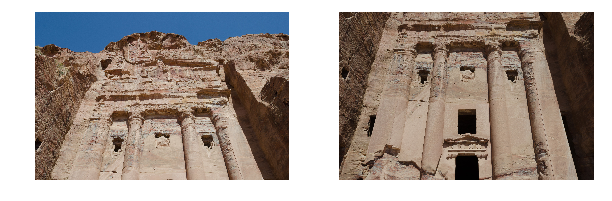
\includegraphics[width=\linewidth]{pano_4_0.png}
    \caption{Petra images\label{fig:petra}}
  \end{subfigure} \\ [0.5ex]  % Small vertical pad

  % Unfiltered ORB features
  \begin{subfigure}{\linewidth}
    \centering
    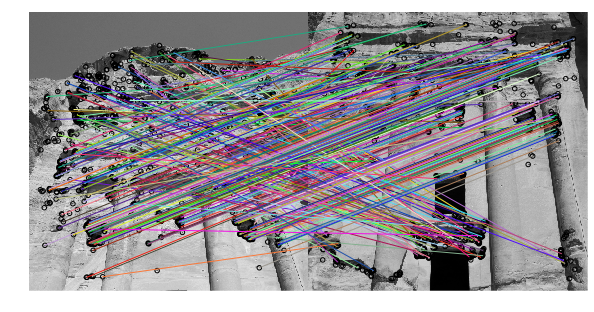
\includegraphics[width=\linewidth]{pano_11_1.png}
    \caption{ORB binary features\label{fig:putativematches}}
  \end{subfigure} \\ [0.5ex]  % Small vertical pad

  % ORB features after RANSAC padding
  \begin{subfigure}{\linewidth}
    \centering
    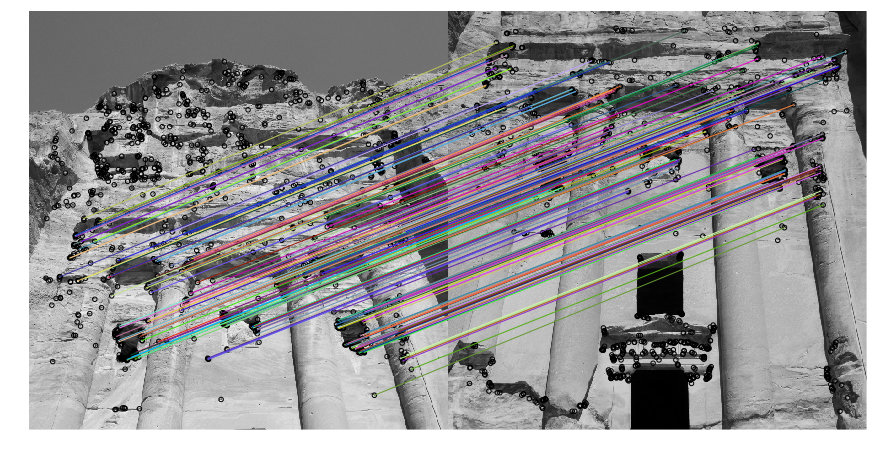
\includegraphics[width=\linewidth]{pano_15_1.png}
    \caption{RANSAC-filtered features\label{fig:matchesfiltered}}
  \end{subfigure} \\ [0.5ex]  % Small vertical pad

  % Correct orientation & simple averaged combination
  \begin{subfigure}{\linewidth}
    \centering
    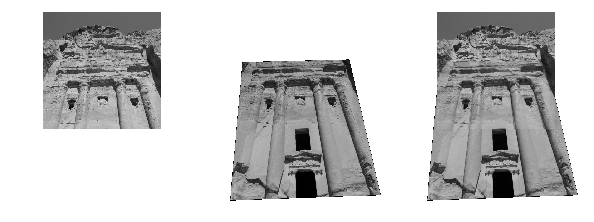
\includegraphics[width=\linewidth]{pano_23_0.png}
    \caption{Warped \& positioned\label{fig:merged}}
  \end{subfigure}
\end{minipage}%
% Right side of figure: Final Enblend result
\begin{minipage}{.5\textwidth}
  \begin{subfigure}{\linewidth}
    \centering
    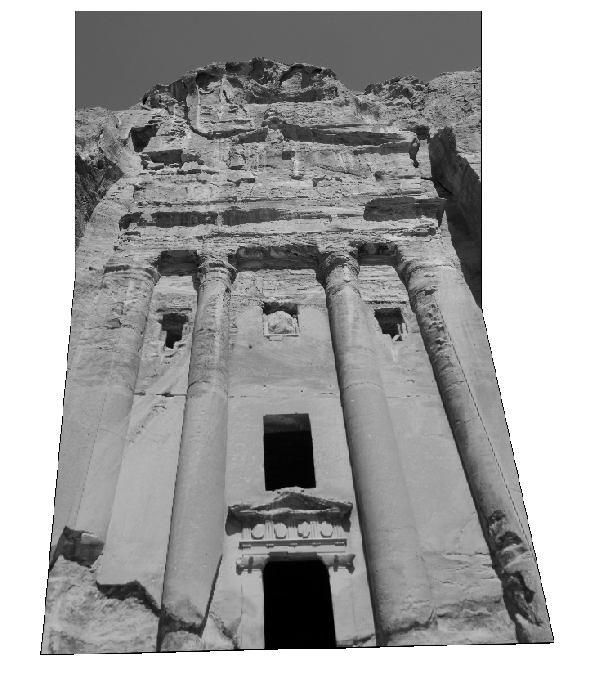
\includegraphics[width=\linewidth]{pano_28_0.png}
    \caption{Final result, combined with Enblend\label{fig:pano}}
  \end{subfigure}
\end{minipage}%
\end{frame}

\caption{An example application of scikit-image: image registration and warping to combine overlapping images. (\subref{fig:petra}): Photographs taken in Petra, Jordan by François Malan. License: CC-BY. (\subref{fig:putativematches}): Putative matches computed from ORB binary features. (\subref{fig:matchesfiltered}): Matches filtered using RANSAC. (\subref{fig:merged}): The second input frame (\textit{middle}) is warped to align with the first input frame (\textit{left}), yielding the averaged image shown on the right. (\subref{fig:pano}): The final panorama image, registered and warped using scikit-image, blended with Enblend.\label{fig:pano_overall}}

\end{figure}